\documentclass{./tex/cslthse-msc}
\usepackage[utf8]{inputenc}
\usepackage[english]{babel}
\usepackage{amsmath}
\usepackage{amsfonts}
\usepackage{amssymb}
\usepackage{amsthm}
%\usepackage{makeidx}
\usepackage{graphicx}
\usepackage[titletoc, header, page]{appendix}
\usepackage{hyperref}


%\geometry{showframe}

\author{
	David Norrestam \\
	{\normalsize \href{mailto:davidnorrestam@gmail.com}{\texttt{davidnorrestam@gmail.com}}}
	\and
	Philip Burenstam Linder \\
    {\normalsize \href{mailto:philip.burenstam.linder@gmail.com}{\texttt{philip.burenstam.linder@gmail.com}}}
}

\title{Hybrid app-development using an existing webapplication}
%\subtitle{A feasibility study}
%\company{The Corporation AB LTD Inc}

%\date{\today}
\date{Month Day, 2015}

\supervisors{Flavius Gruian, \href{mailto:Flavius.Gruian@cs.lth.se}{\texttt{Flavius.gruian@cs.lth.se}}}{Albin Svensson, \href{mailto:albin.svensson@trialbee.com}{\texttt{albin.svensson@trialbee.com}}}
%\supervisor{John Deer, \href{mailto:jdeer@company.com}{\texttt{jdeer@company.com}}}
\examiner{Flavius Gruian, \href{mailto:flavius.gruian@cs.lth.se}{\texttt{flavius.gruian@cs.lth.se}}}


\acknowledgements{
If you want to thank people, do it here, on a separate right-hand page. Both the U.S. \textit{acknowledgments} and the British \textit{acknowledgements} spellings are acceptable.
}

\theabstract{
This document describes the Master's Thesis format for the theses carried out at 
the Department of Computer Science, Lund University. 

Your abstract should capture, in English, the whole thesis with focus on the problem and solution in 150 words. It should be placed on a separate right-hand page, with an additional \textit{1cm} margin on both left and right. Avoid acronyms, footnotes, and references in the abstract if possible.

Leave a \textit{2cm} vertical space after the abstract and provide a few keywords relevant for your report. Use five to six words, of which at most two should be from the title.
}

\keywords{android, hybrid, application, app-development, webapplication, integrating, webview}

%% Only used to display font sizes
\makeatletter
\newcommand\thefontsize[1]{{#1 \f@size pt\par}}
\makeatother
%%%%%%%%%%

\begin{document}
\makefrontmatter
\chapter{Introduction}
% Add text here that motivates this thesis, perhaps a quick intro 
\section{Background}
\subsection{A brief explanation of Android, hybrid applications and PhoneGap}
Android is operating system used on a wide range of devices, such as a mobile device or tv device. Coding android applications is done in the programming language Java. Code for android can be written in the official Android development environment, Android studio, but other development environment is also available. 
\newline
\newline
Android software development kit (SDK) provides the programmer with a number of tools. Such as a debugger, library, device emulator, and documentation.  
\newline
\newline
A hybrid application is a native application which is partially written with web technologies. I.e HTML5, CSS and JavaScript. The part of the application written with web technologies runs within a browsers engine in a so called WebView. A web application running in a browser does not have access to a device native functions such as the bluetooth. However a website running within a WebView can through interaction with the application's native code access a device native functions.
\newline
\newline
PhoneGap is a framework for developing mobile applications. The code is written with web technologies, the code is compiled to different platform, such as Android or IOs, specific code. The resulting application is a hybrid application. An example of a mobile application built in PhoneGap is wikipedia's mobile application.  

\section{Problem formulation}
The aim of this project is to evaluate two different development methods for encapsulating an existing web application in an Android mobile application, in order to give the web application access to the mobile's native functions. An example of such a native function would be accessing the camera of a mobile phone. It is important that the logic on the web application can be written in a general way (non-platform dependant) adapting to the device accessing the web application. This way, the method used to encapsulate the web application is easy to replace, with minimum effect on the logic of the web application. 
\newline\newline
As the first development method, the mobile application will be built natively (in Java for android). As the second method, the mobile development framework PhoneGap will be used. The methods will be evaluated and compared from a developers perspective, with the preconditions defined section \ref{section-preconditions}

\subsection{Preconditions}\label{section-preconditions}
The study is done from a company's perspective and is based on the following prerequisites:
\begin{itemize}
\item There are only a few developers, three or less
\item There is already an existing web-application that is to be used by the mobile-application
\item The company has a need and/or desire to extend the functionality of it's web-application with native functions
\item The company's developer or developers has no prior knowledge of mobile application development
\end{itemize}

When examining the methods, the focus has been restrained to the following developing aspects
\begin{itemize}
\item Modularisation in a way so that its easy to add functionality
\item The web application should be loosely coupled with native code
\item Maintainability (easy to update in case of API change)
\end{itemize}
\section{Contribution statement}
Throughout this work we have been working together all the time. When writing code we often been pair programming and if not we have reviewed each others code afterwards. Researching has also been done together. It is therefore impossible to point to whom has done what in this thesis since all our work has been done together. 

%Om du har utför examensarbetet tillsammans med en annan student ska det i rapporten tydligt framgå vem av er som har gjort vad, både i fråga om arbetet och rapporten.

\section{Terminology}
\begin{description}
  \item[Mobile application] \hfill \\
    Refers to the application being developed, excluding code loaded from remote        websites.
  \item[Web application] \hfill \\
    If nothing else is specified it refers to the client-side of the web application.
  \item[Development methods] \hfill \\
    Refers (in the context of this paper) to the methods of mobile application          development being evaluated, i.e. using the development framework PhoneGap or       writing native Android code.
  \item[Native function] \hfill \\
     A hardware function which a device has. For example mobile with a camera and GPS have native functions when writing mobile software or applications to get access to the camera or it's GPS.
\end{description}


\chapter{Approach}
This chapter begins with a presentation of the method used in this thesis, followed by a section explaining the demo application developed as part of the method. The last section contains a presentation of recent articles on the subject. 
\section{Method}
In order to compare the two development methods (described in problem formulation), we have tried using them both to 
In order to research the problem formulation of this paper, a practical approach has been used. The two different development methods (as described in problem formulation) have been used in a practical development process. The aim of the development has been to develop an architecture allowing independent web application code and mobile-application code to be written.
\newline\newline
Apart from just developing architectures using the different methods, a demo-application was developed. The application had the same function requirements for both development methods. 

This also put requirements on the web application, it had to confirm to a certain standard for communication with the mobile application in order for both applications to be able to use it. 
\newline\newline
Another important aspect of the method, and a major part of the results found in this paper is the process of researching questions arising during the process. Examples of this can be questions regarding strengths and weaknesses of the method at hand, but also questions of a more basic nature, such as the behavior of function calls between the layers (web and mobile), are they synchronous?

\subsection{Demo application}
The demo application consists two mobile applications developed using the different development methods. The web application which is used in the mobile applicaitons is a simple form with a text field, an image field and a location field.
\newline\newline
When running on a computer in a web browser the web application make use of the computer's camera and the web browser's own function to get the computers location. To see the web application please visit: https://pollux-server.herokuapp.com/
\newline\newline
The two mobile applications make use of the web application described above. To get the image for the web application form the mobile application makes use of the mobile's native camera function or uploads an image from the mobile's memory storage. To get the location the mobile applications makes use of the mobile's native GPS function. 
\newline\newline
Aplication source code can be found at:
\newline
Web application: https://github.com/Albin-trialbee/pollux-server
\newline
PhoneGap application: https://github.com/DavidNorrestam/pollux-phonegap
\newline
Native Android mobile application: https://github.com/buren-trialbee/pollux/

\subsection{Recent work}
In “Native vs Hybrid / PhoneGap App Development Comparsion” (http://www.comentum.com/phonegap-vs-native-app-development.html), research made by Comentum 360, they estimate the development cost for a small to medium size project in Android native development and in PhoneGap. They estimate that both methods would cost the same, about 10-20 thousand dollars. They also mention the limitations of using PhoneGap, describing that hybrid apps (like PhoneGap) relies on a development framework and the provided features when building a mobile application. Hence, if the framework is not up to date with the latest new features, the developer will not be able to partake of the features until the framework is updated. Their conclusion of this is that if an application is dependent on many native features a hybrid application may have limitations. 
\newline
\newline
TJ VanToll author of the book "JQuery UI in Action" writes amongst other things in the article, “The State of Hybrid Mobile Development” (http://developer.telerik.com/featured/the-state-of-hybrid-mobile-development/), about the history of hybrid mobile development using web technologies. He points out that there has been a lot of issues such as debugging and lack of tools. Two things which made companies like Facebook and LinkedIn abandon developing native applications with web technologies. Troubles, he today believes mostly are solved with all the progress which has been made the recent years.

\chapter{Evaluation}
The evaluation has been divided into two different parts, one for each development method being evaluated. In 
\section{Native android} \label{android}
\subsection{Modularisation}
The android application has a lot of different responsibilities, apart from communicating with the native API and web application, it also has to contain the necessary activity threads to function as an application. A modularisation of the code into as small sections as possible has been the goal of the architecture being developed. The different responsibilities can be summarized as:

\begin{itemize}
\item Communication with the Android native API
\item Communication with the web application
\item Handling activity lifecycle
\item Starting activities for results (ex. the camera)
\end{itemize}


To conform to this modularisation, the architecture as figure \ref{caption-android-architecture} has been proposed. This divides the application into separate modules with a single responsibility, where the bridges responsibility is to handle communication between modules and add necessary logic for simple tasks such as casting of objects or performing calculations. 


\begin{figure}[ht!]
    \centering
    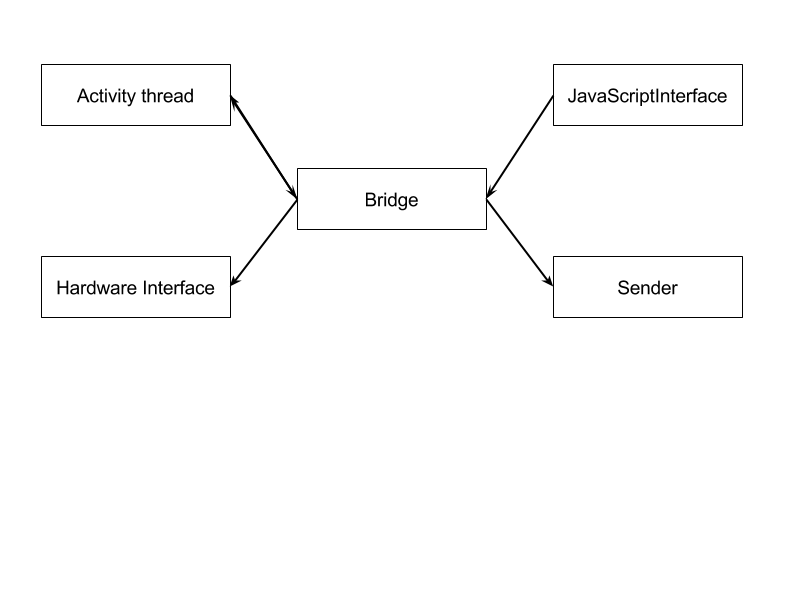
\includegraphics[width=120mm,natwidth=800,natheight=600]{./img/androidStructure.png}
    \caption{Architecture of the android application\label{caption-android-architecture}}
\end{figure}


(Add section describing function flow between java and javascript)

\begin{figure}[ht!]
    \centering
    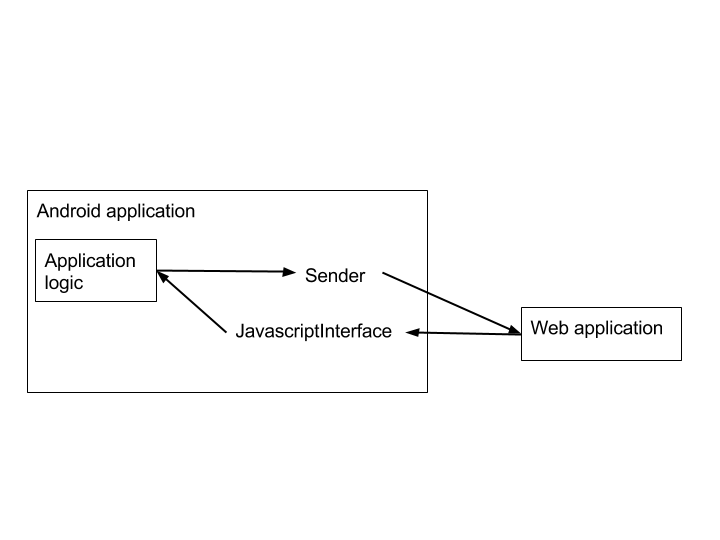
\includegraphics[width=120mm,natwidth=720,natheight=540]{./img/androidFlow.png}
    \caption{Function flow of the android application\label{caption-android-flow}}
\end{figure}

\subsection {Function calls between Java and JavaScript}
Calling javascript functions from Java is done using the function loadUrl on the WebView containing the web application. This was deducted to be an asynchronous method call, through practical tests in the development phase of this paper. 
\newline\newline
(Add section containing example test here)
\newline\newline
When calling java functions on the exposed javaScriptInterface object from javascript, the behavior of the function call is a bit more obscure. Due to the single-threaded nature of javascript, function calls are synchronous when called in a normal fashion.
\newline\newline
(Add section containing example test here)
\newline\newline
( However, by the usage of AJAX, the function calls may behave asynchronous on the web application side. Then the question arises, can two functions be executed in parallel on the android side, or is the execution of the jsInterface functions limited to being handled by a single thread. )<--Needs to be researched to stay here.

Utvärdering (Evaluation) bör beskriva den metod som används för att utvärdera din metod, inklusive experimentuppställning.
\section{Web application} 
\subsection{Results}
\subsubsection{Separating business logic from device specific logic}
An requirement on the web application is the ability to separate the business logic from device specific logic. This can be done with an adapter pattern. To set the right adapter a different method is used for Android and PhoneGap. The usage of this pattern ensures a natural way of modularising the code and separating all business logic from logic related to device-specific communication, the business logic is thus independent of the running device. 

\subsubsection{Encapsulating the web application in native Android application}
When encapsulating the web application when writing the mobile application in native Android code is done by the use of a WebView. When the web application is loaded in the native layer through a WebView an object is made available to the web application on which the web application can use to send messages to the native layer. Therefore checking if the web application is running within a WebView can be done by:
\begin{verbatim}
if(typeof Android !== 'undefined'){
 adapter = new AndroidAdapter()
}
\end{verbatim}
Where “Android” is the object made available to the web application by the native layer and can be used to invoke native functions.

\subsubsection{Encapsulating the web application in a PhoneGap application}
Here the same type of text as the chapter above shall be written


An overview of the recommended architecture for the web application can be seen below, where the internal structure of the mobile application is irrelevant. 

\begin{figure}[ht!]
    \centering
    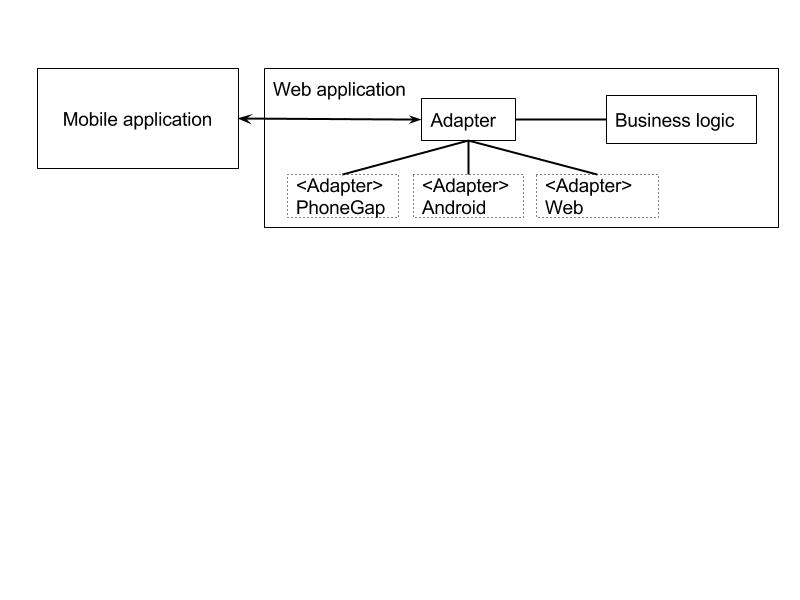
\includegraphics[width=140mm,natwidth=800,natheight=600]{./img/webAppFlow.jpg}
    \caption{Web application function calling flow \label{caption-web-flow}}
\end{figure}

\subsubsection{Communication between web application and mobile application}
(this chapter shall be rewritten)
Another functionality raising concerns regarding dependency is the communication between the web application and mobile application. The adapters dependency on the mobile application code is inevitable, unless communication can be made in a standardized way, and all devices expose methods conforming to an interface. The same thing goes for communication back to the web application, however in this case, the web application can expose a javascript function handling device callbacks, and as long as all devices are able to invoke javascripts in the web application, communication is independent apart from the name of the callback function. Ok that was not entirely true, in order for communication to be independent, all calls to the device must include the name of a callback function that will later be passed to the device callback function in the web application, which then relays callback data correctly. Also, the dependency on standardized callback data is still there, however this is a wanted behavior, as the data being sent back should be of the same type.

\section{PhoneGap}

\subsection{Communicatating between PhoneGap (native) layer and the web application}

\begin{figure}[ht!]
    \centering
    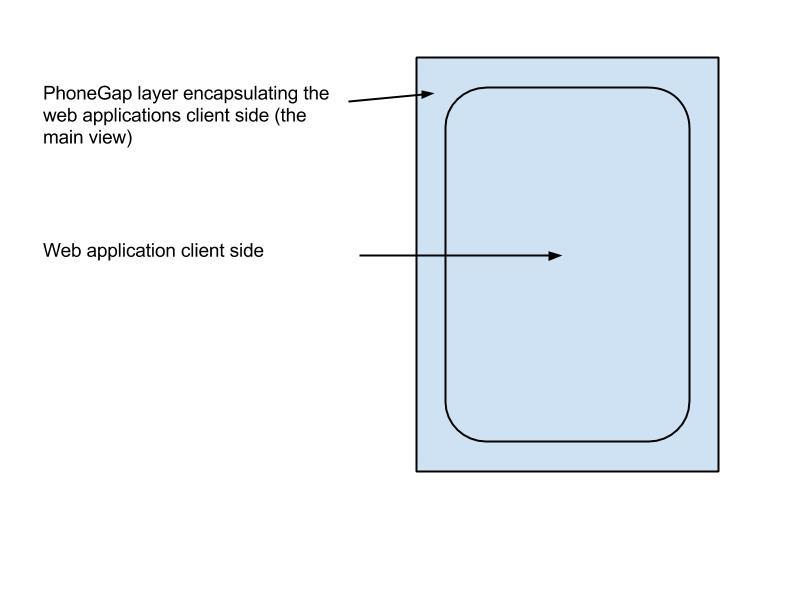
\includegraphics[width=120mm,natwidth=800,natheight=600]{./img/phonegap.jpg}
    \caption{The PhoneGap layer encapsulating the web application\label{overflow}}
\end{figure}


\subsubsection{Encupsulating the web application in an iFrame}
The remote web application is loaded in an iFrame, whilst PhoneGap logic is running in the main view (see picture). The default response header for a web page contains rules regarding same-origin policy, which disallows the webpage from being embedded in an iFrame on another web page, unless they have the same origin. The response header therefore needs to be modified, in order to allow web pages with other origins to load the webpage in an iFrame. 
This is done differently depending on the web development framework, in the framework Rails this can be done by: 

\begin{verbatim}
HomeController  < ApplicationController
  after_action :allow_iframe
  private
    def allow_iframe
      response.headers.except! 'X-Frame-Options'
     end
\end{verbatim}

Function calling from the web application is done by the use of postMessage on the parent window, the PhoneGap-layer listens to these messages by the use of an event listener. A request call from the web application is a message containing two key-value pairs: “type” and “callback”. The value of “type” specifies which native function the web application desires data from. The value of “callback” is used by the PhoneGap-layer when sending the data back to the web application. This is done with the predefined method deviceCallback on the adapter in the web application:

\begin{verbatim}
Adapter.deviceCallback(nativeData, calbackName);
\end{verbatim}

This way the PhoneGap layer only need to know in which format the data should be in, nothing else. 
\begin{figure}[ht!]
    \centering
    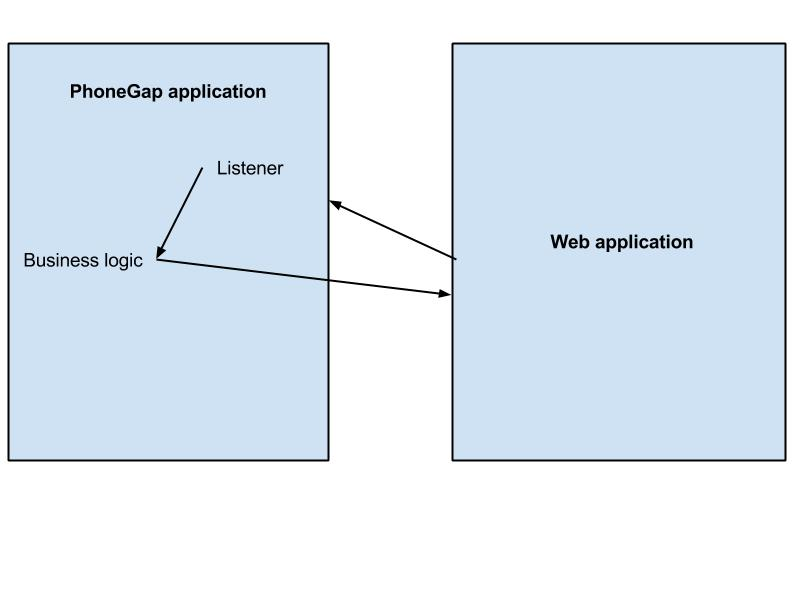
\includegraphics[width=120mm,natwidth=800,natheight=600]{./img/phoneGapFlow.jpg}
    \caption{PhoneGap function calling flow \label{caption-phonegap-flow}}
\end{figure}
\newline
The web application sends a message which is received by the listener in the PhoneGap application. The listener calls the function specified by the message, and passes on the callback to it. Upon completion the resulting data is passed to the web application, along with the callback, 

\subsubsection{Using polling in the PhoneGap plugin inAppBrowser}

inAppBrowser is a PhoneGap plugin which basically opens a browser “in the application”. By using this plugin to embed the remote web application, communication between the windows becomes different than when using an iFrame. Sending data from the PhoneGap-layer to the web application can be done by using the inAppBrowser function “executeScript”, which, in the inAppBrowser, executes the javascript passed as argument.
The communication back from the web application is more complicated. One example of how to do it is by the use of polling variables in the web application using executeScript. For further reading the following blog article: “Cross Window Communication With Cordova’s inAppBrowser” (http://blogs.telerik.com/appbuilder/posts/13-12-23/cross-window-communication-with-cordova\%27s-inappbrowser) by TJ VanToll is recommended. 
\newline\newline
Other ways requires deeper technical web development knowledge. For more suggested methods read the support request https://issues.apache.org/jira/browse/CB-4897.

\subsubsection{Using a third party plugin}
PhoneGap supports custom plugins. This opens up the ability for companies to write their own plugins or make use of other third party plugins.
\newline\newline
There is a PhoneGap plugin written by the corporation Wizcorp which claims it enables communication between the PhoneGap layer and web application. However despite extensive effort it never worked in this project. A ananswered support question (25/3-2015) can be seen at https://github.com/Wizcorp/phonegap-plugin-wizViewManager/issues/77. 

\subsection{Demo}
The demo code can be found at https://github.com/DavidNorrestam/pollux-phonegap. In the demo the communication between the PhoneGap layer and the web application is done by using an iFrame and postMessage, see chapter above. The most interesting files in the repository are found in:

\begin{description}
  \item[www/js/receiver.js] \hfill \\
    All the logic for receiving a message from the web application
  \item[www/js/device.js] \hfill \\
    Logic for some native functions and loading the web application
  \item[www/index.html] \hfill \\
    The html code for the mobile application view
\end{description}

\chapter{Discussion}
\subsection{Developing in Android}
\subsubsection{Getting started}
\subsubsection{Debugging}
Debugging when using the Android Studio IDE is a fairly simple process. For developers familiar with Java-debugging, the process is as good as similar, apart from the fact that the code is run on an emulator, or real device, rather than on directly by the JVM. Complications do occur when the application contains a WebView or other browser and the aim is the debug both the web and java code. However, with the help of the chrome inspect tool, the web code is easily debugged, and debugging of communication in between Java and JavaScript is easiest made by a combination of this tool and the built-in debugger. 
\subsection{Developing in PhoneGap}
\subsubsection{Getting started}
Getting familliar with PhoneGap is quite confusing. This resulting in that it took around two days to set up a working development environment that felt comfortable. There were a few reasons for this. You need to install a lot dependencies such as nodejs, a server-side runtime environment, and Apache Cordova. Apache Cordova can be described as the engine of PhoneGap. There is also several different ways to develop the mobile application. You can compile and build the app for testing yourself or use a cloud service like https://build.phonegap.com/ to compile your code for you. The relationship between Apache Cordova and PhoneGap is also initially confusing. It was also very difficult to find a good “Getting started” guide.

\subsubsection{Adding and debbuging native functionality}
The documenation is clear and feels complete. If you require extra help the PhoneGap community is very active and there is lots of help to get from blog posts and Q\&A sites such as stackoverflow.com. This make’s it very simple to make use of the mobile’s native functions. 
\newline
\newline
When using mobile native function a plugin need to be added to the project. The plugin can be supported by PhoneGap, a third party plugin or a plugin you write yourself. A PhoneGap plugin for using the mobile’s cambera is added by writing the following bash command in your project root folder:
\begin{verbatim}
$ cordova plugin add org.apache.cordova.camera
\end{verbatim}
The code for taking a picture with the camera in your mobile application is:
\begin{verbatim}
navigator.camera.getPicture( cameraSuccess, cameraError, cameraOptions );
\end{verbatim}
Where “cameraSucess” and “cameraError” is a callback function. 
\newline
\newline
To build and run the project on your mobile for testing you run in the root folder of your project:
\begin{verbatim}
$ cordova build android; 
$ cordova run android;
\end{verbatim}

For the debbuging the mobile application you can open desktop browser and where you can see the HTML, CSS and JavScript code and debugg the same way as a web application debugging is done in a web browser inspector. More can be read about debugging a PhoneGap application at https://github.com/phonegap/phonegap/wiki/Debugging-in-PhoneGap.  



Thoughts:
 - The development of the architectures of the different methods can not be ensured to be entirely independent. Thus the results might vary depending on the order the development methods get evaluated. Also they're both reliant on the webapplication, if this one gets developed early on, they will have to conform to its standards, thus limiting the developers freedom. 

Positive / negative experiences
\begin{itemize}
    \item We are both skilled in java
    \item Very basic knowledge of webprogramming
    \item Our experience of developing in android
    \item Our experience of developing using phonegap
    \item Other
\end{itemize}

Diskussion (Discussion) möjliggör en längre diskussion och tolkning av resultaten från utvärderingsavsnittet, inklusive extrapoleringar och/eller förväntade resultat. Här passar det också att beskriva positiva och negativa erfarenheter relaterade till det arbete du har utfört.

\chapter{Conclusions}
Slutsatser (Conclusions) bör sammanfatta dina slutsatser och redogöra för möjliga förbättringar och eventuella rekommendationer.
\end{document}